\documentclass[osajnl,twocolumn,showpacs,superscriptaddress,10pt]{revtex4-1}


%PAQUETES<<<<<<<<<<<<<<<<<<<<<<<<<<<<<<<INICIO
\usepackage{dcolumn}% Align table %columns on decimal point
\usepackage{bm}% bold math
%
%Paquete de Idioma
\usepackage[spanish]{babel}
%
%Codificación Alfabeto
\usepackage[utf8]{inputenc}
%
%Codificación de Fuente
\usepackage[T1]{fontenc}
%
%Índice
\usepackage{makeidx}
%
%Gráficos3
\usepackage{graphicx}
\usepackage{subfig}
% \usepackage{longtable}
%\usepackage{xcolor} 
%
%Matemática
\usepackage{amsmath}
\usepackage{amsfonts}
\usepackage{amssymb}
%\usepackage{amstext} 
%
%Estilo de Página Numeración superior
%\pagestyle{headings}
%
%Hiperlinks \href{url}{text}
\usepackage[pdftex]{hyperref}
%
%Graficos y tablas
\usepackage{multirow}
%\usepackage{multicol}
\usepackage{float}
\usepackage{booktabs}
%
\decimalpoint
%\bibliographystyle{IEEEtran}
%\bibliography{IEEEabrv,mybibfile}
%
%
%PAQUETES<<<<<<<<<<<<<<<<<<<<<<<<<<<<<<<INICIO

\begin{document}
%SIGNOS
%TILDE -> \' <vocal>
%TEXTO_NEGRITA -> \textbf{<texto>}
%TEXTO_ITALICA -> \textit{<texto>}
%TEXTO_SUBRAYADO -> \underline{<texto>}

%TITTULO DEL ARTICULO
\title{\Huge IoT Proyecto Uno -  Vehículo Inteligente Transportador de Paquetes  - Arquitectura de Computadores y Ensambladores 2 }
%AUTORES DEL ARTICULO

\author{\newline Airton Yelstin de León Obando (201602836) - Rol: Analítico}
\affiliation{Grupo No.7 - Universidad de San Carlos de Guatemala, Escuela de Ciencias y Sistemas
}%

\author{\newline Edgar Mauricio Gómez Flores, (201114340) Rol: Infraestructura del Producto}%
\affiliation{Grupo No.7 - Universidad de San Carlos de Guatemala, Escuela de Ciencias y Sistemas
}%
\author{\newline Jurgen Andoni Ramirez Ramirez, (201404179) Rol: Conectividad}%
\affiliation{Grupo No.7 - Universidad de San Carlos de Guatemala, Escuela de Ciencias y Sistemas
}%
\author{\newline Josue Eduardo Abelarde Perez, (201602890) Rol: Smart-APP}%
\affiliation{Grupo No.7 - Universidad de San Carlos de Guatemala, Escuela de Ciencias y Sistemas
}%
\date{Septiembre 2020}



%INICIO DE DOCUMENTO<<<<<<<<<<<<<<<<<<<<<<<<<<<<<<<<<
\begin{abstract}
\title {resumen}
En este proyecto se pretende hacer uso del concepto de IoT aplicado a un buzón inteligente junto con un vehículo transportador de paquetes. El vehículo se diseñó de tal forma que cuando se detecte un nuevo paquete pueda moverse a través de una ruta y entregar dicho paquete a su destino, lo anterior haciendo uso de diversos sensores digitales, dispositivos electrónicos y mecánicos a su vez recolectando y procesando la información obtenida por el vehículo en la nube para que se mueva entre el punto de partida y su destino controlando sus movimiento y funciones proveyendo información útil para el usuario final.
\end{abstract}
\maketitle{}
\section{INTRODUCCIÓN}
Al hablar de introducir el concepto de IoT es este proyecto principalmente se habla de la importancia de recolectar datos y hacer uso de estos datos provenientes de cualquier objeto de la vida diaria cuya utilidad aumenta significativamente al convertir estos datos en información relevante y de interés en su funcionamiento, de tal manera que este objeto expande las funciones para las que fue originalmente creado. Ahora que se cuenta con un buzón inteligente para desinfectar paquetes se considera la implementación de un vehículo transportador inteligente capaz de medir su peso y transportar los paquetes desde el buzón del usuario, su punto de partida, hasta la puerta del usuario, su destino. El vehículo es capaz de seguir una linea coloreada que marca la ruta de su recorrido, además como parte de sus funciones este puede detectar obstáculos en su trayectoria y detener la marcha hasta que este obstáculo sea removido, una vez ha llegado a su destino el vehículo envía los datos a la nube, los almacena en una base de datos y una aplicación para dispositivos móviles advierte al usuario de su llegada así como otros datos importantes, tales como: la hora de partida desde el buzón y su hora de entrega junto con el peso del paquete recibido. Una vez entregado el paquete el vehículo procede a regresar al buzón en reversa y colocarse en el punto de espera hasta recibir un nuevo paquete. Por último el usuario es capaz de hacer que el vehículo transportador entre en estado activo o inactivo. Entre la información de relevancia para el usuario se tiene un historial de:
\begin{itemize}
    \item[$\bullet$]\textbf{Ubicación del vehículo.}
    \item[$\bullet$]\textbf{Estado del vehículo.}
    \item[$\bullet$]\textbf{Cantidad de paquetes entregados.}
    \item[$\bullet$]\textbf{Total de obstáculos detectados.}
    \item[$\bullet$]\textbf{Peso promedio de los paquetes entregados.}
    \item[$\bullet$]\textbf{Tiempo promedio que ha tardado en llegar el vehículo desde el buzón hasta el punto de entrega.}
    \item[$\bullet$]\textbf{Tiempo promedio que ha tardado en llegar el vehículo desde el punto de entrega de regreso hasta el buzón.}
    
\end{itemize}

Todos puntos listados anteriormente pueden ser vistos desde la pantalla principal de \textbf{'Dash Board'} de la aplicación para dispositivos móviles inteligentes, estos serán actualizados al momento que se llevan a cabo las tareas, o sea en tiempo real, permitiendo al usuario saber cual es el estado del vehículo en todo el momento y lugar que desee.

\section{Prototipo de Diseño}
Ya que el objetivo de este vehículo es transportar los paquetes recibidos desde el buzón inteligente hasta su destino se ha optado por un diseño que cuenta con cuatro ruedas para un movimiento eficaz a través de la ruta que deberá seguir, además considerando la variedad de tipos de objetos que transportará se tiene una carcasa solida prefabricada como chasis donde se colocaran los demás componentes electrónicos, mecánicos y sensores, \textbf{véase figura 1}.


\begin{figure} [H] \centering 
\caption{Boceto de diseño}
%IMAGENS DE CHASIS
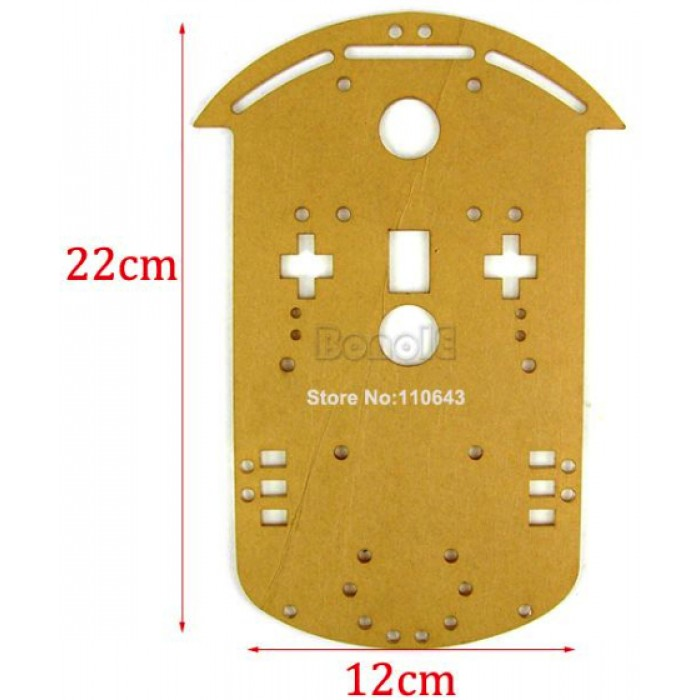
\includegraphics[width=0.5\textwidth]{chasis.jpg} 
Esta estructura está hecha de un material sintético con tal de que este sea mas ligero.
\end{figure}


La estructura es importante al momento de colocar los demás componentes, en la \textbf{figura 2} se puede apreciar el conjunto de componentes principales que conforman al vehículo.

\begin{figure} [H] \centering 
\caption{Componentes Pricipales de vehículo}
%IMAGEN DE COMPONENTES DE VEHICULO
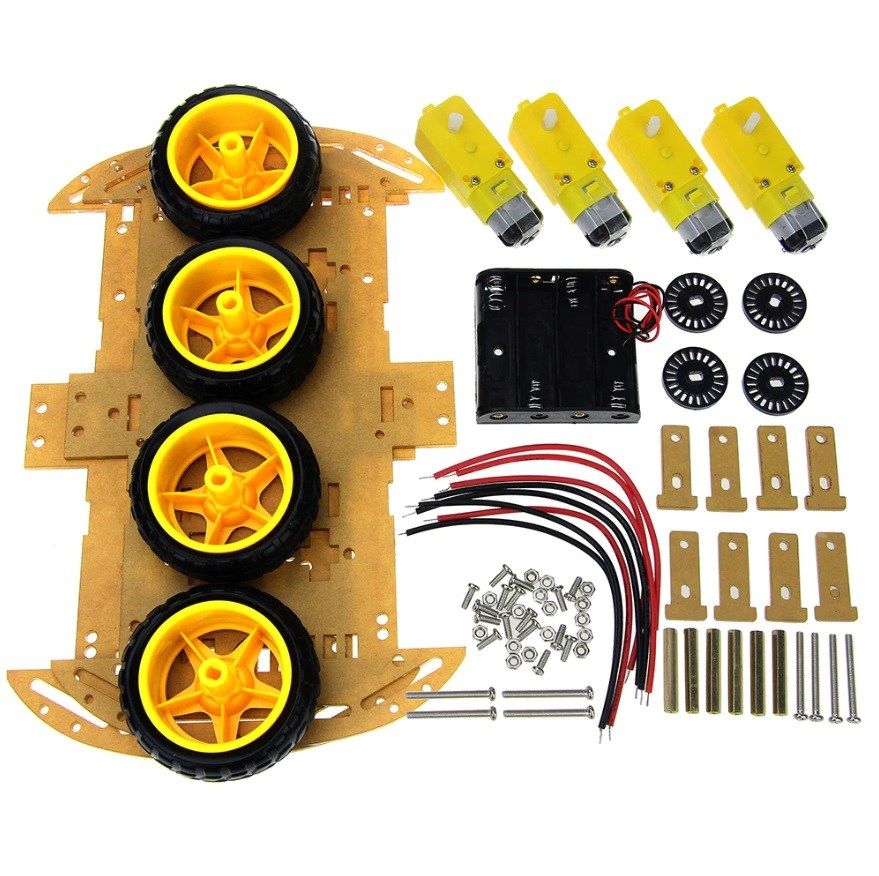
\includegraphics[width=0.5\textwidth]{componentes.jpg}
\end{figure}

Por ultimo se puede observar en la \textbf{figura 3} una vista de estos componentes principales ensamblados que finalmente se ven para que le vehículo este en condición de realizar sus labores.

\begin{figure} [H] \centering 
\caption{Vehículo Armado}
%IMAGEN DE COMPONENTES PRINCIPALES MONTADOS
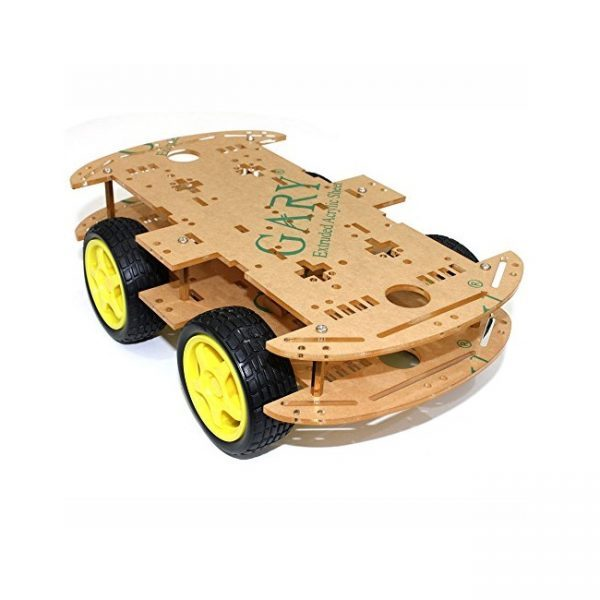
\includegraphics[width=0.5\textwidth]{armazon.jpg} 
Armazón, motores y ruedas ensambladas.
\end{figure}

\section{Famework de Productos Inteligentes Conectados}
\subsection{Infraestructura del Producto}
\subsubsection{Hardware:}
\begin{itemize}
    \item[$\bullet$]\textbf{Armazón prefabricada} de para chasis vehículo transportador.
    \item[$\bullet$]Módulo de balanza HX711
    \item[$\bullet$]1 Batería de 9V.
    \item[$\bullet$]1 Broche para batería de 9V con plug DC
    \item[$\bullet$]\textbf{Cuatro moto-reductores con motores DC} para producir movimiento del vehículo.
    \item[$\bullet$]\textbf{Cuatro Ruedas Plásticas} para hacer posible el movimiento de vehículo.
    \item[$\bullet$]\textbf{Tornillos y tuercas M3} para ensamblar la armazón del vehículo.
    \item[$\bullet$]\textbf{4 Baterías AA de 1.5V} como fuente de energía para vehículo.
    \item[$\bullet$]\textbf{Caja plástica} contenedora para baterías de alimentación.
    \item[$\bullet$]Dispositivo de \textbf{Módulo WiFi}.
    \item[$\bullet$]\textbf{Arduino Uno.}
    \item[$\bullet$]\textbf{Cables} para conexiones.
    \item[$\bullet$]\textbf{Cautín} para realizar soldaduras.
    \item[$\bullet$]\textbf{Estaño.}
    \item[$\bullet$]\textbf{1 Mini protoboard de 170 puntos} para armar circuitos digitales.
    \item[$\bullet$]\textbf{Plataforma} para colocar los paquetes que el vehículo debe transportar.
    \item[$\bullet$]\textbf{Módulo Puente H L298 }para control de Motores DC.

\end{itemize}
\subsubsection{Software}
    Se han diseñado y programado los algoritmos necesarios para la recolección de datos de interés sobre el estado del vehículo inteligente, los paquetes que transporta, las tareas que este realiza a través de cada uno de los sensores integrados, además se incluyen las funciones de control del vehículo sobre las que el usuario tiene acceso desde su dispositivo móvil por medio de el microcontrolador ARDUINO para su posterior trasmisión y procesamiento en la nube. Todo ello usando el lenguaje de programación C++, usado por estos microcontroladores.
    
\subsection{Sensores}
\begin{itemize}
    \item[$\bullet$]\textbf{Sensor de peso} para determinar la presencia de nuevos paquetes.
    \item[$\bullet$]\textbf{2 Sensores ultrasónicos HC-SR04} para saber cuando se encuentra un nuevo obstáculo.
    \item[$\bullet$]4 Sensores de Línea Perpendicular TCRT5000.
\end{itemize}
\subsection{Conexión}
    La comunicación utilizada entre el vehículo inteligente y el usuario final es a través de una conexión inalámbrica \textbf{WiFi}. El dispositivo arduino recolecta la información pertinente para ser codificada y transmitida desde el vehículo a través del módulo \textbf{WiFi} realizando peticiones \textbf{HTTP} con el servidor a través de una \textbf{API/REST} que se encargará de almacenar, procesar y transmitir la información codificada al dispositivo móvil del usuario desde la base de datos en la nube. Ver figura 4. \newline
\begin{figure} [H] \centering 
\caption{Representación de conexión}
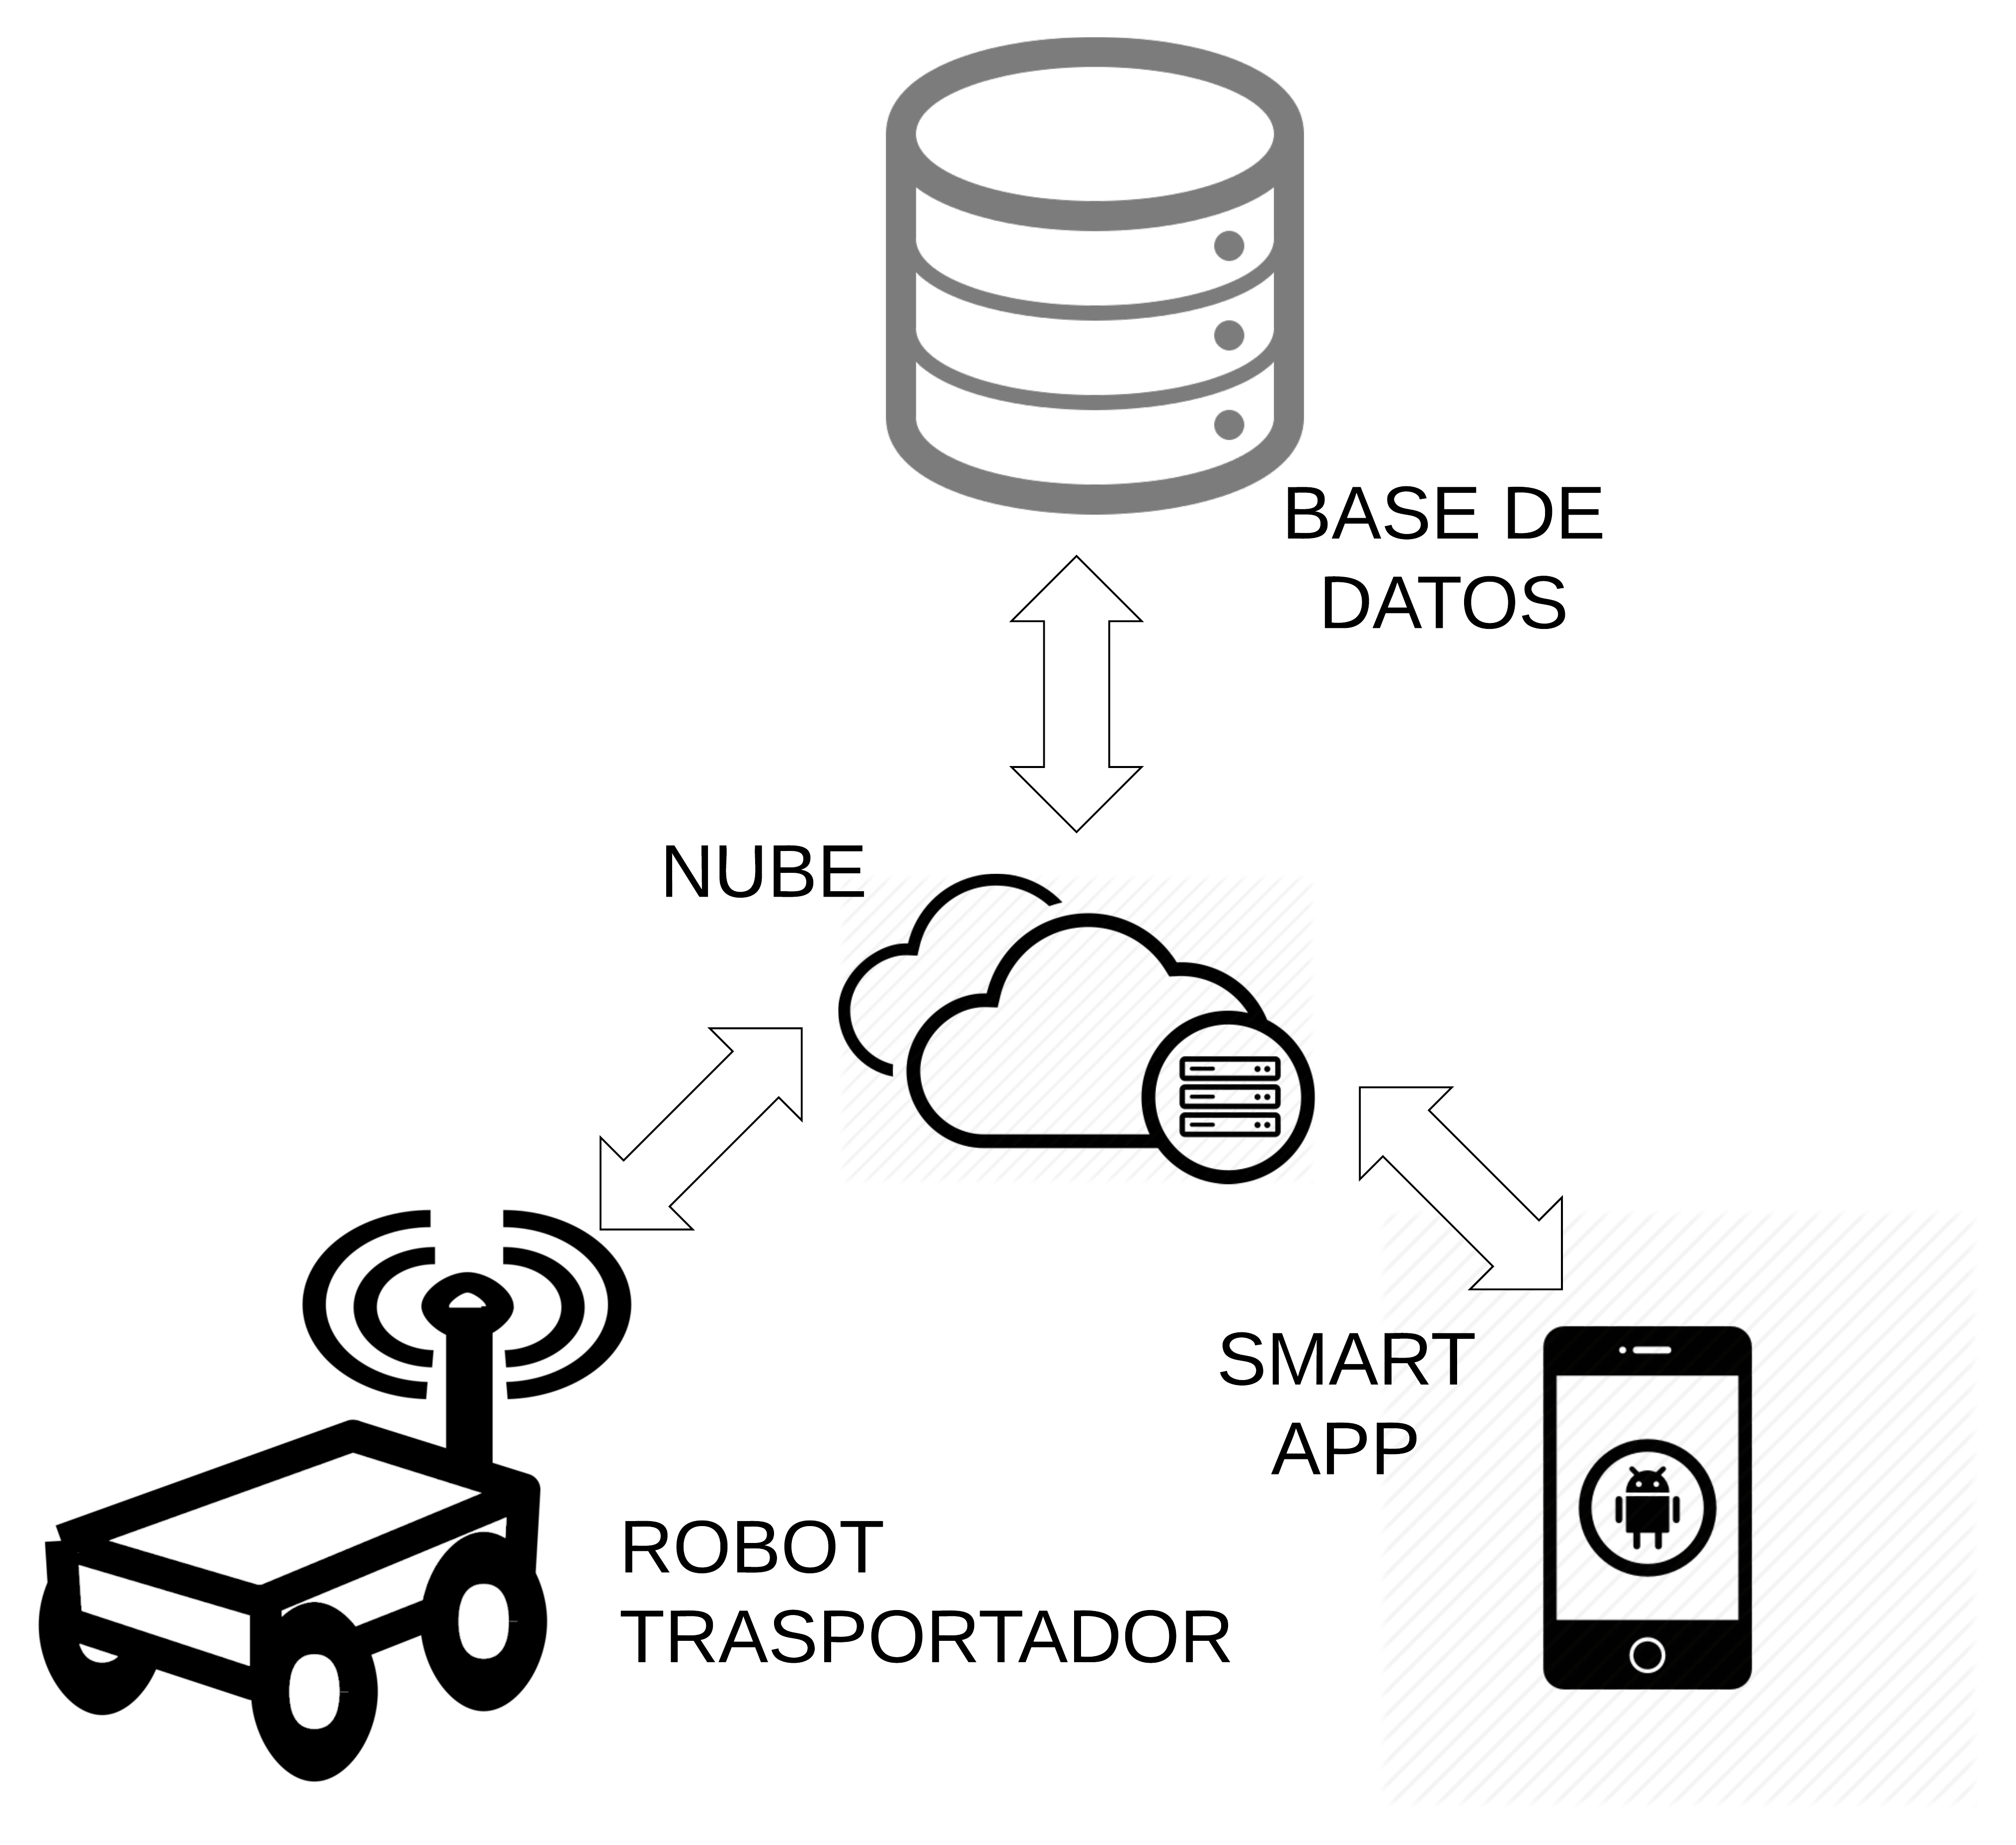
\includegraphics[width=0.5\textwidth]{conexion.png} 
La comunicación entre el vehículo inteligente, el servidor y el usuario será bidireccional, ya que el usuario es capaz de realizar acciones sobre el vehículo.
\end{figure}
\subsection{Análisis}
    En este proyecto de IoT el vehículo transportador recolecta información constantemente sobre su estado y el de los paquetes que este recolecta, además el usuario tiene la capacidad de ver esta información desde su dispositivo, pero la información se procesa para que le sea útil al usuario, en este caso en análisis se hace en la característica de visualizar promedios de peso de los paquetes, tiempos de entrega y el conteo del total de paquetes entregados exitosamente. Además, la capacidad de hacer que el vehículo entre en modo de inactividad pues se debe procesar y decodificar la información enviada a través del dispositivo hasta el vehículo.
\subsection{Smart APP}
    Como se menciono en varias ocasiones el usuario puede conectarse al vehículo inteligente a través de su dispositivo móvil, esta aplicación esta dirigida a dispositivos móviles que usan el sistema operativo \textbf{Android}, esta aplicación móvil cuenta con varias características, pero la principal es su DashBoard donde se pueden visualizar varios datos de interés para el usuario, a continuación se muestran y detallas las funciones de la aplicación.
    
\begin{figure} [H] \centering 
\caption{PANTALLA 1 ( Dash Board en Aplicación móvil )}
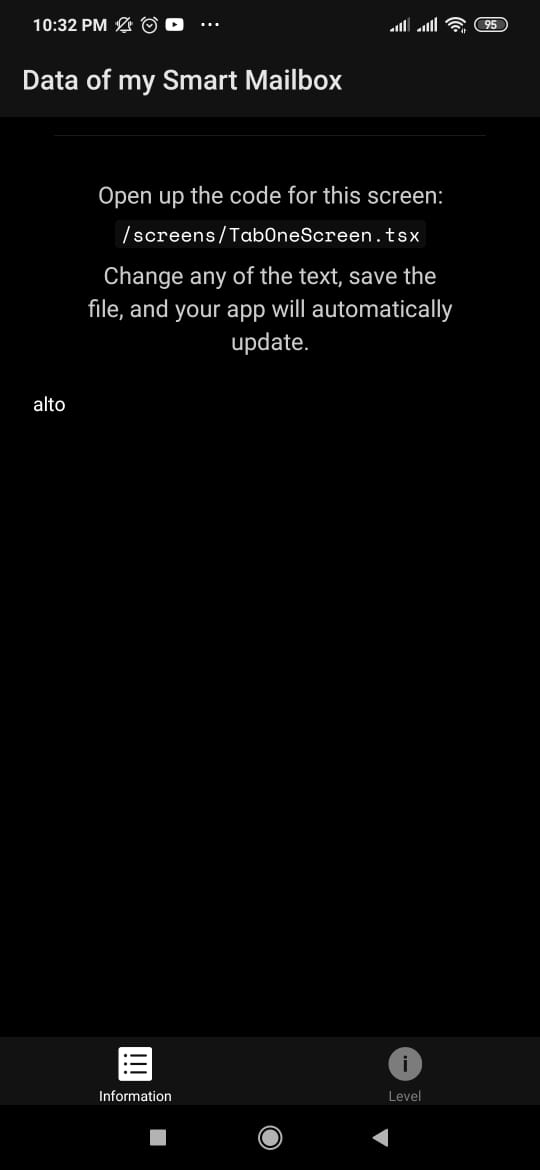
\includegraphics[width=0.4\textwidth]{img1.jpeg} 
\\
Este es el aspecto del la pantalla principal del Dash Board en la aplicación móvil. Cada uno de los valores presentados: Estado, Ubicación, Tiempo Promedio, Tiempo Promedio ida, Tiempo Promedio Regreso, Total contador y Total obstáculos se actualiza cada vez que el vehículo recibe alguna paquete y realiza su entrega.
Para que los cambios sean visibles se debe Presionar el botón \textbf{Actualizar}.\\
Si se desea hacer que el vehículo entre en estado activo o inactivo se deberá presionar los botones \textbf{Activar} o \textbf{Desactivar}, respectivamente.
\end{figure}
\\

\begin{figure} [H] \centering 
\caption{PANTALLA 2 ( Notificaciones de Aplicación Móvil )}
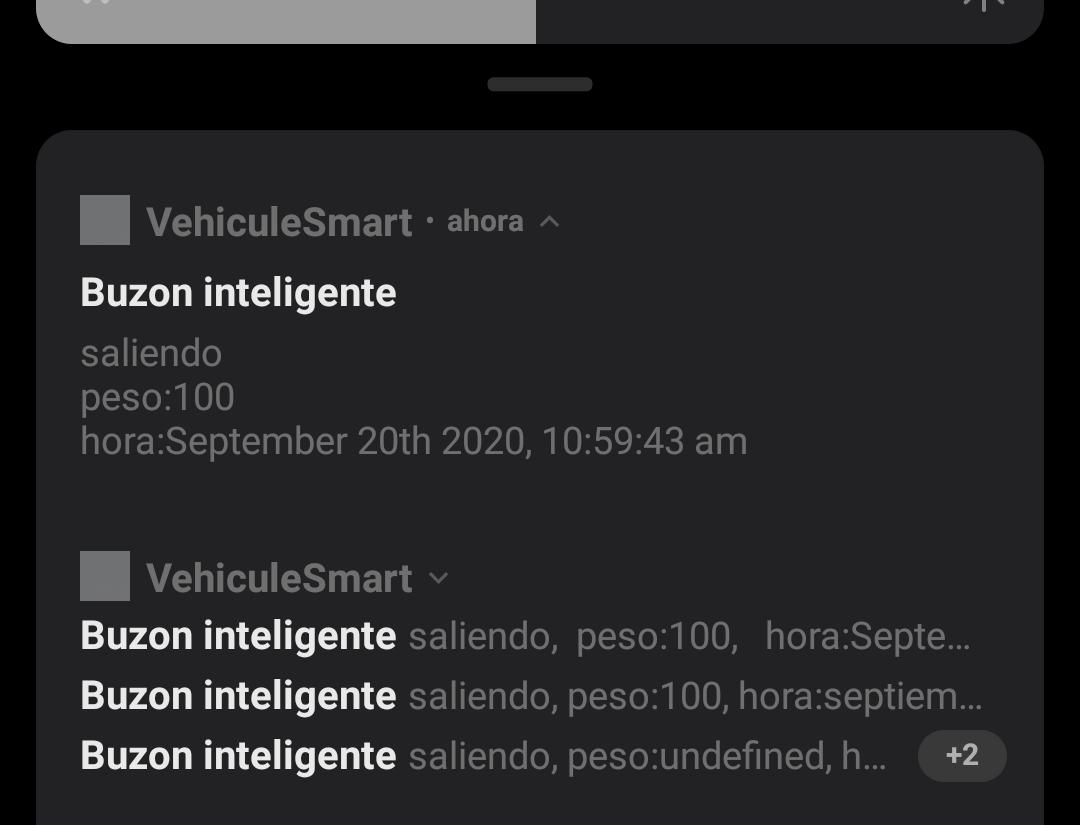
\includegraphics[width=0.4\textwidth]{img2.jpeg} 
\\
Cada vez que el vehículo detecte que un nuevo paquete ha sido recibido el vehículo procede a enviar una notificación emergente en el dispositivo del usuario, para advertirle que la entrega del paquete a su destino esta en proceso.
\end{figure}
\section{Vídeos de funcionamiento}
\begin{itemize}
    \item[$\bullet$]Video1: https://youtu.be/-WbvX138Zik
\end{itemize}

\end{document}
